\chapter{Reporting} \label{ch:reporting}
A graphical user interface was created to report the transducer readings to an end user in a friendly format. In order to achieve this an Arduino Leonardo compatible Beetle board was used to communicate with a PC via UART communications so that the analogue transducer measurements could be sent to the GUI, the trip switch status could be read and finally to give the user control of the trip override switch.

\section{Design} \label{sec:rep_design}
To interface the Arduino's pins with the transducer output the ground pin on the Arduino had to be connected to the common ground plate of the analogue circuitry, and protection diodes had to be added in parallel with each individual pin. A single $\SI{4.7}{V}$ zener diode was placed as close to each of the input pins as possible to protect against both overvoltage and undervoltage conditions. Once a voltage greater than the threshold breakdown voltage of the zener diode is applied at the input pin the zener diode would start conducting and thus clamp the input to the pin \cite{zenerboi}. The only limitation of this choice of clamping circuit is that it relies on the slope of the breakdown voltage curve of the diode model chosen.\vspace{4mm} \newline The high level representation of the Arduino program flow can be seen in Figure \ref{subfig:arduino_code_flow}, the Arduino served the purpose of supplying the switching frequency of the charge pump, reading the status of the trip switch, providing the functionality of resetting the trip switch status and reading the analogue outputs of all of the transducers. As the state of the SR latch in Chapter \ref{sec:switch} was undefined on startup for the cases where the system was connected to the PC before it was turned on, additional functionality was added to ensure that the reset signal would go high for a few milliseconds on the initialisation of the Arduino code. The python program flow can be seen in Figure \ref{subfig:python_code_flow}, this program entails the design of the GUI that the end user would use to interface with the analogue circuitry. \vspace{4mm} \newline The Arduino and python programs interacted with each other via serial communication setup with a 19200 Baud rate and 8N1 configuration, the list of commands and responses for the communication protocol is specified in Tables \ref{tab:commsprotocal1} and \ref{tab:commsprotocal2}. The basic user command and response functionality was achieved by manually entering the first and second bytes to the serial line as per Appendix D, however additional code had to be written to allow the reading of the state of the trip switch status and allowing the user to reset the trip switch via a button press. 

\section{Measurements} \label{sec:rep_meas}
The transducer levels were measured by using the analogue pins of the Arduino and initialising them as input pins. To ensure the reported measurements remained accurate within the required tolerance specified in Chapter \ref{sec:trans} the ADC measurements had to be re-calibrated. Firstly several measurements were taken comparing the emulated voltage level to the deduced output of each transducer. Linear regression was applied to the measurements displayed in Table \ref{tab:voltagetransducercalibrated} for the voltage transducer, and Equation \ref{eq:vtranscalibrated} was obtained relating the ADC voltage to the deduced output voltage, with Equation \ref{eq:vtranscalibratedrms} displaying the formula that was used to convert the analogue reading to an RMS voltage. 
\begin{align}
  V_{load} &= 7.348V_{adc}+0.259 \label{eq:vtranscalibrated} \\
  V_{load(rms)} &= \sqrt{2}(7.348\frac{5(adc\_value)}{1023}+0.259) \label{eq:vtranscalibratedrms} 
\end{align}
The same procedure was followed for the phase and current transducers and Equations \ref{eq:itranscalibratedrms} and \ref{eq:ptranscalibratedrms} were obtained from the results in Tables \ref{tab:currenttransducercalibrated} and \ref{tab:phasetransducercalibrated}
\begin{align}
  I_{load(rms)} &= \sqrt{2}(73.455313\frac{5(adc\_value)}{1023}+ 1.181447) \label{eq:itranscalibratedrms} \\
  \phi_{load} &= 36\frac{5(adc\_value)}{1023}-3 \label{eq:ptranscalibratedrms} 
\end{align}

\begin{figure}[h]
 \footnotesize
 \centering
    \begin{subfigure}[]{0.49\textwidth}
              \centering
  		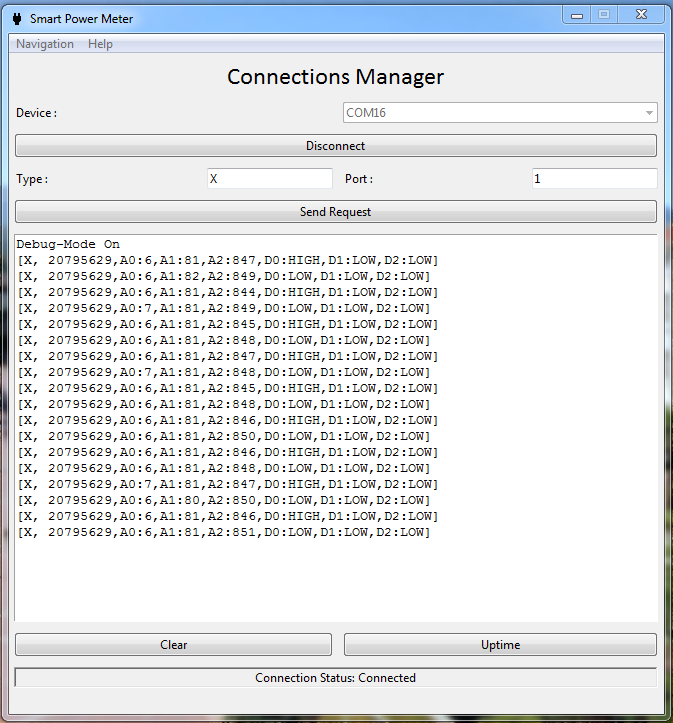
\includegraphics[width=1\linewidth]{./Figures/screengrab_gui_debug.PNG}
		    \caption{} \label{subfig:screengrab_gui_debug}
     \end{subfigure}
          \begin{subfigure}[]{0.49\textwidth}
             \centering
  		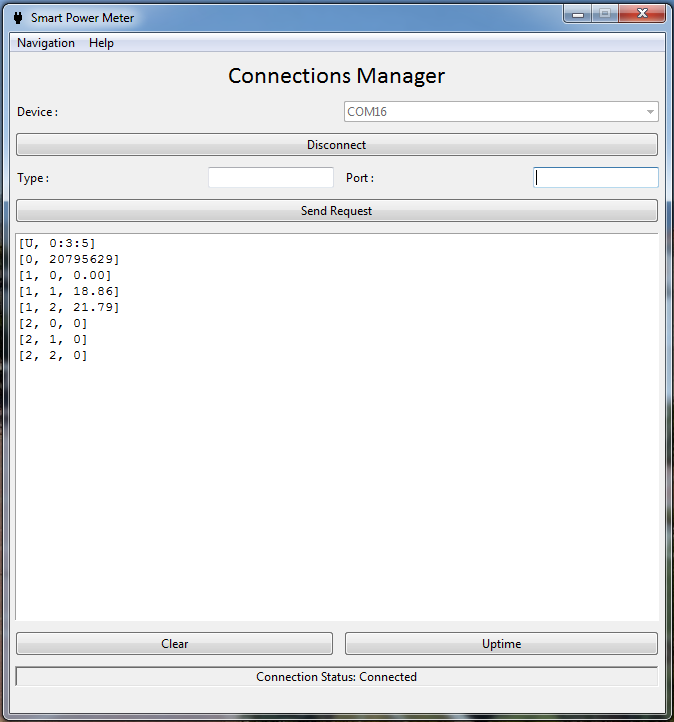
\includegraphics[width=1.0\linewidth]{./Figures/screengrab_gui_other.PNG}
		   \caption{ } \label{subfig:screengrab_gui_other}
     \end{subfigure}
   \caption[Screengrabs of the basic GUI functionality]{Screengrabs of the basic GUI functionality: (a) Debug functionality. (b)  Basic functionality command responses. }
    \label{fig:gui_results}
 \end{figure}

\section{Results} \label{sec:rep_results}
The basic GUI functionality is displayed in Figure \ref{subfig:screengrab_gui_other} showing the response to various user commands as listed in Table \ref{tab:commsprotocal1}, with the debug functionality output shown in Figure \ref{subfig:screengrab_gui_debug}. For a complete overview of the GUI functionality please refer to Chapter \ref{sec:extra_func} for the additional functionality as well as displaying of the switch trip status and the related trip override button.
 
\section{Summary and implementation}
The user interface displaying the connection status to the Arduino, the trip switch status and override as well as the measurements from the transducers was successfully implemented in this design. A communication protocol was also established between the Arduino and graphical python code as to standardise the communication between the two interfaces. Finally the transducer readings were calibrated as to ensure accurate reporting of the measurements displayed, with clamping diodes added to the inputs of the Arduino to protect against overvoltage surges.

\begin{figure}[h]
 \footnotesize
 \centering
    \begin{subfigure}[]{0.4\textwidth}
              \centering
  		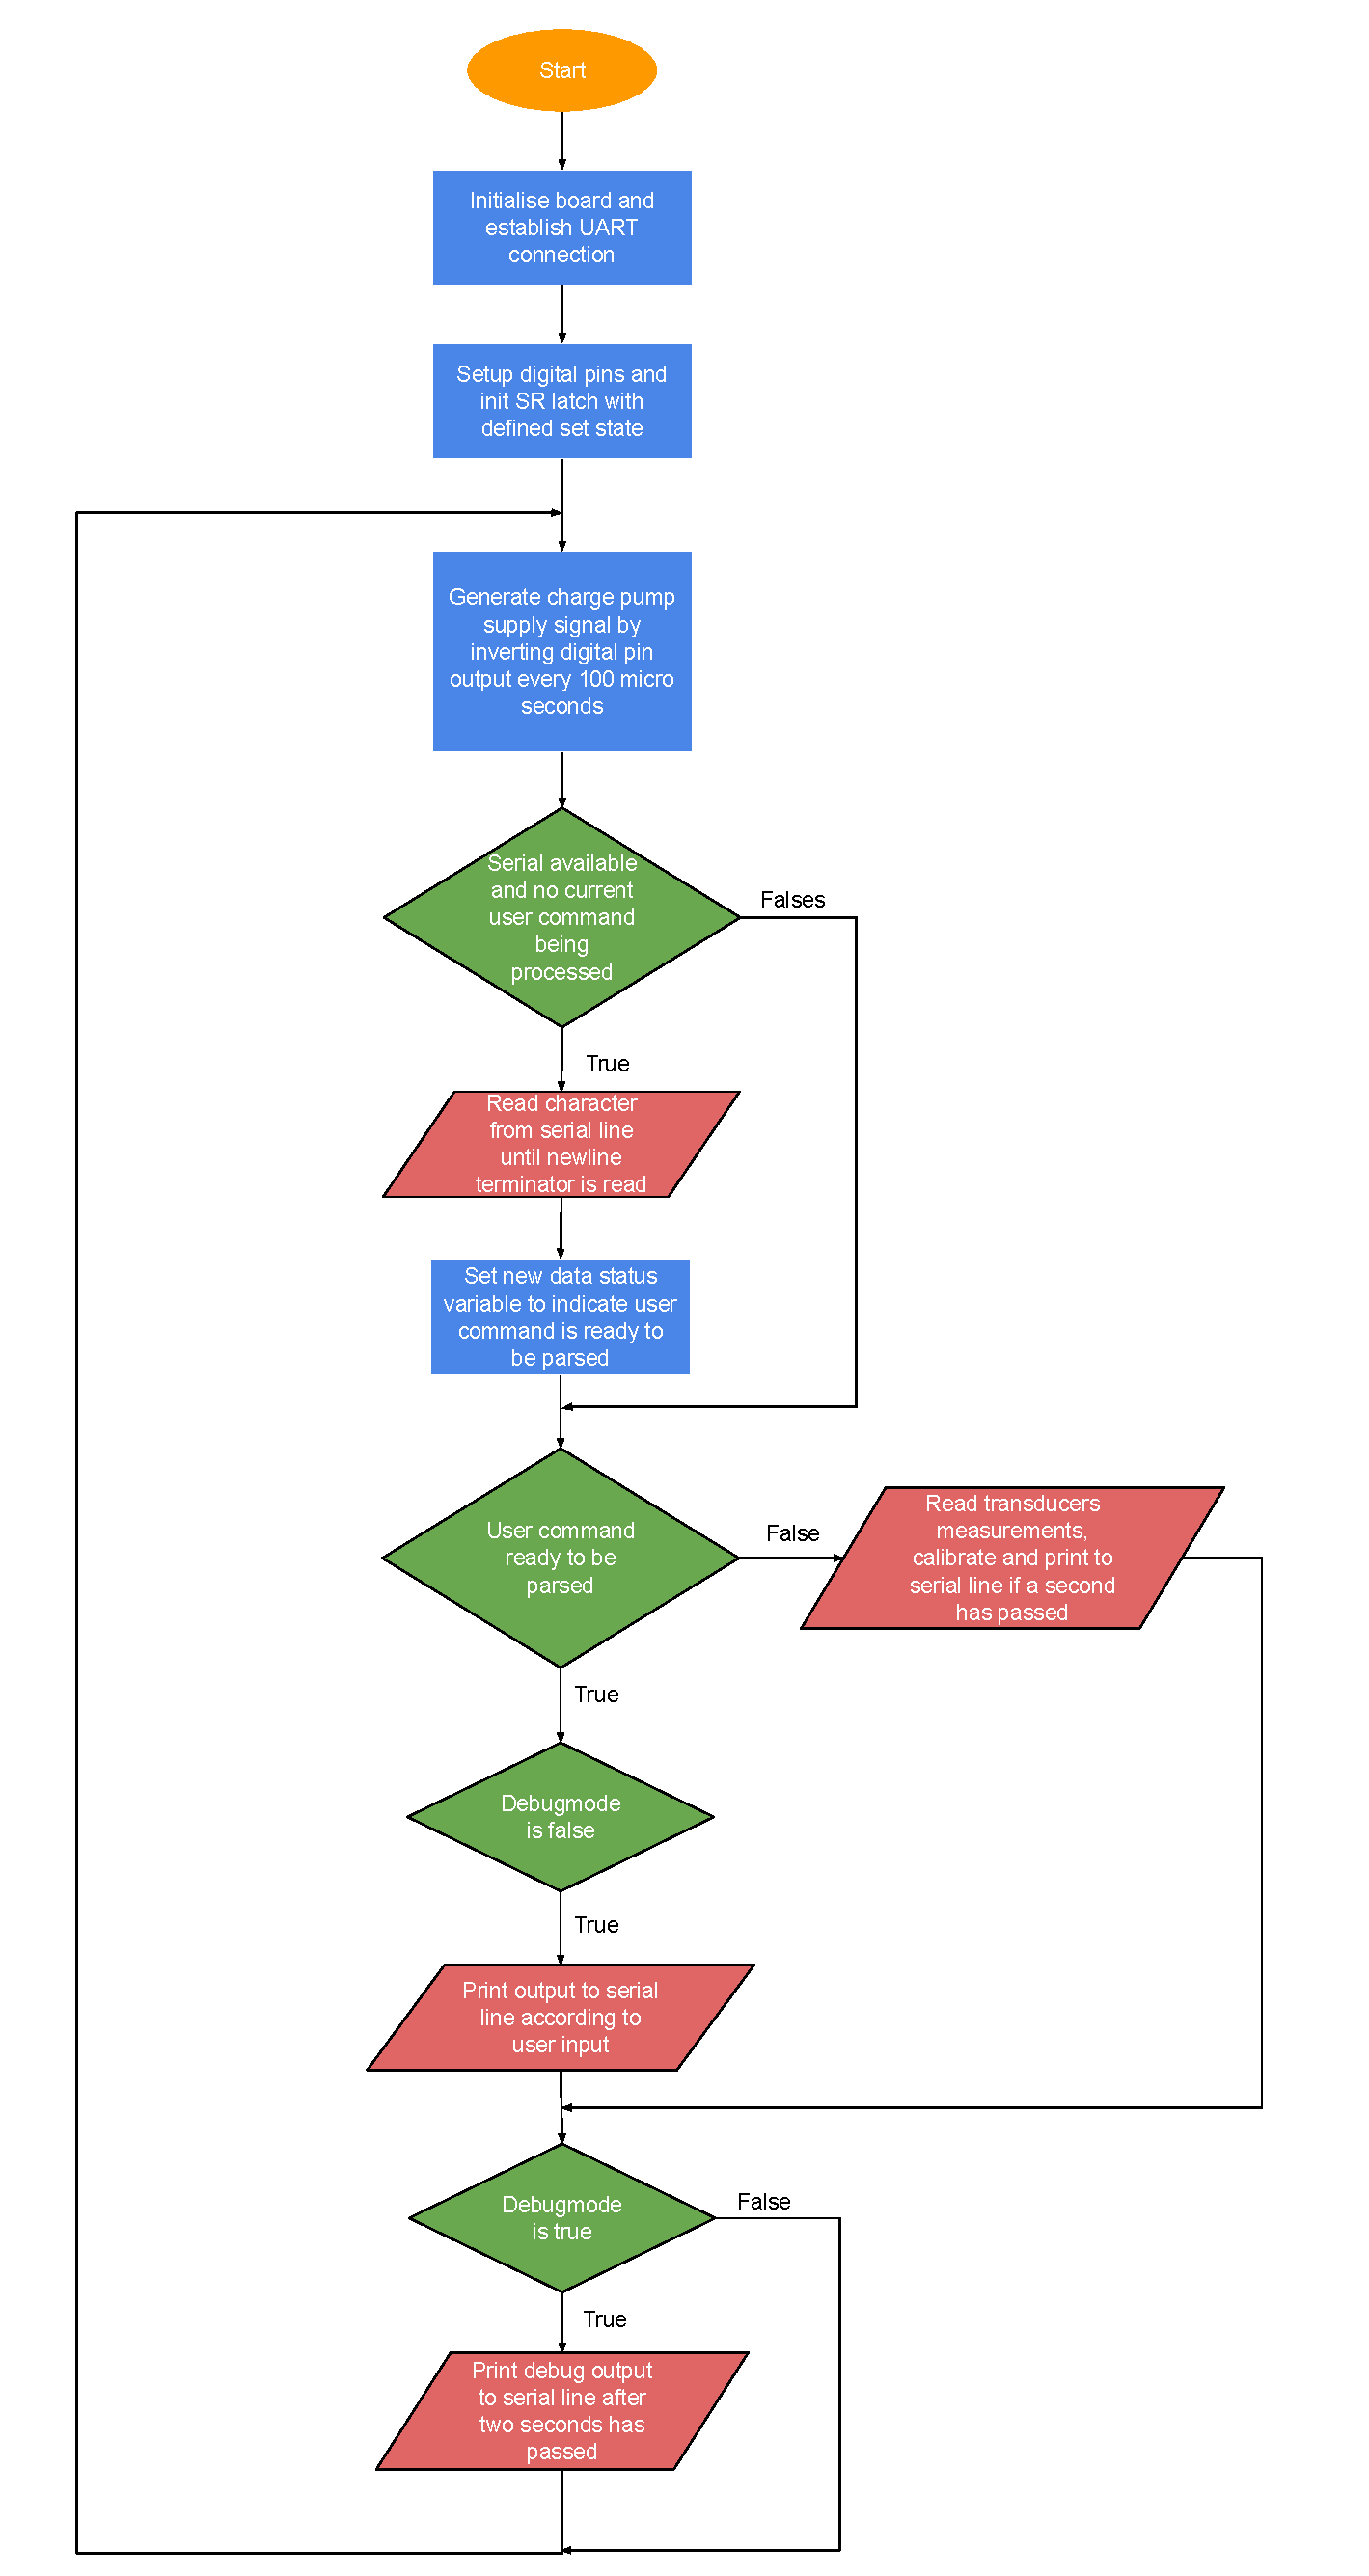
\includegraphics[width=1\linewidth]{./Figures/arduino_code_flow.pdf}
		    \caption{} \label{subfig:arduino_code_flow}
     \end{subfigure}
          \begin{subfigure}[]{0.4\textwidth}
             \centering
  		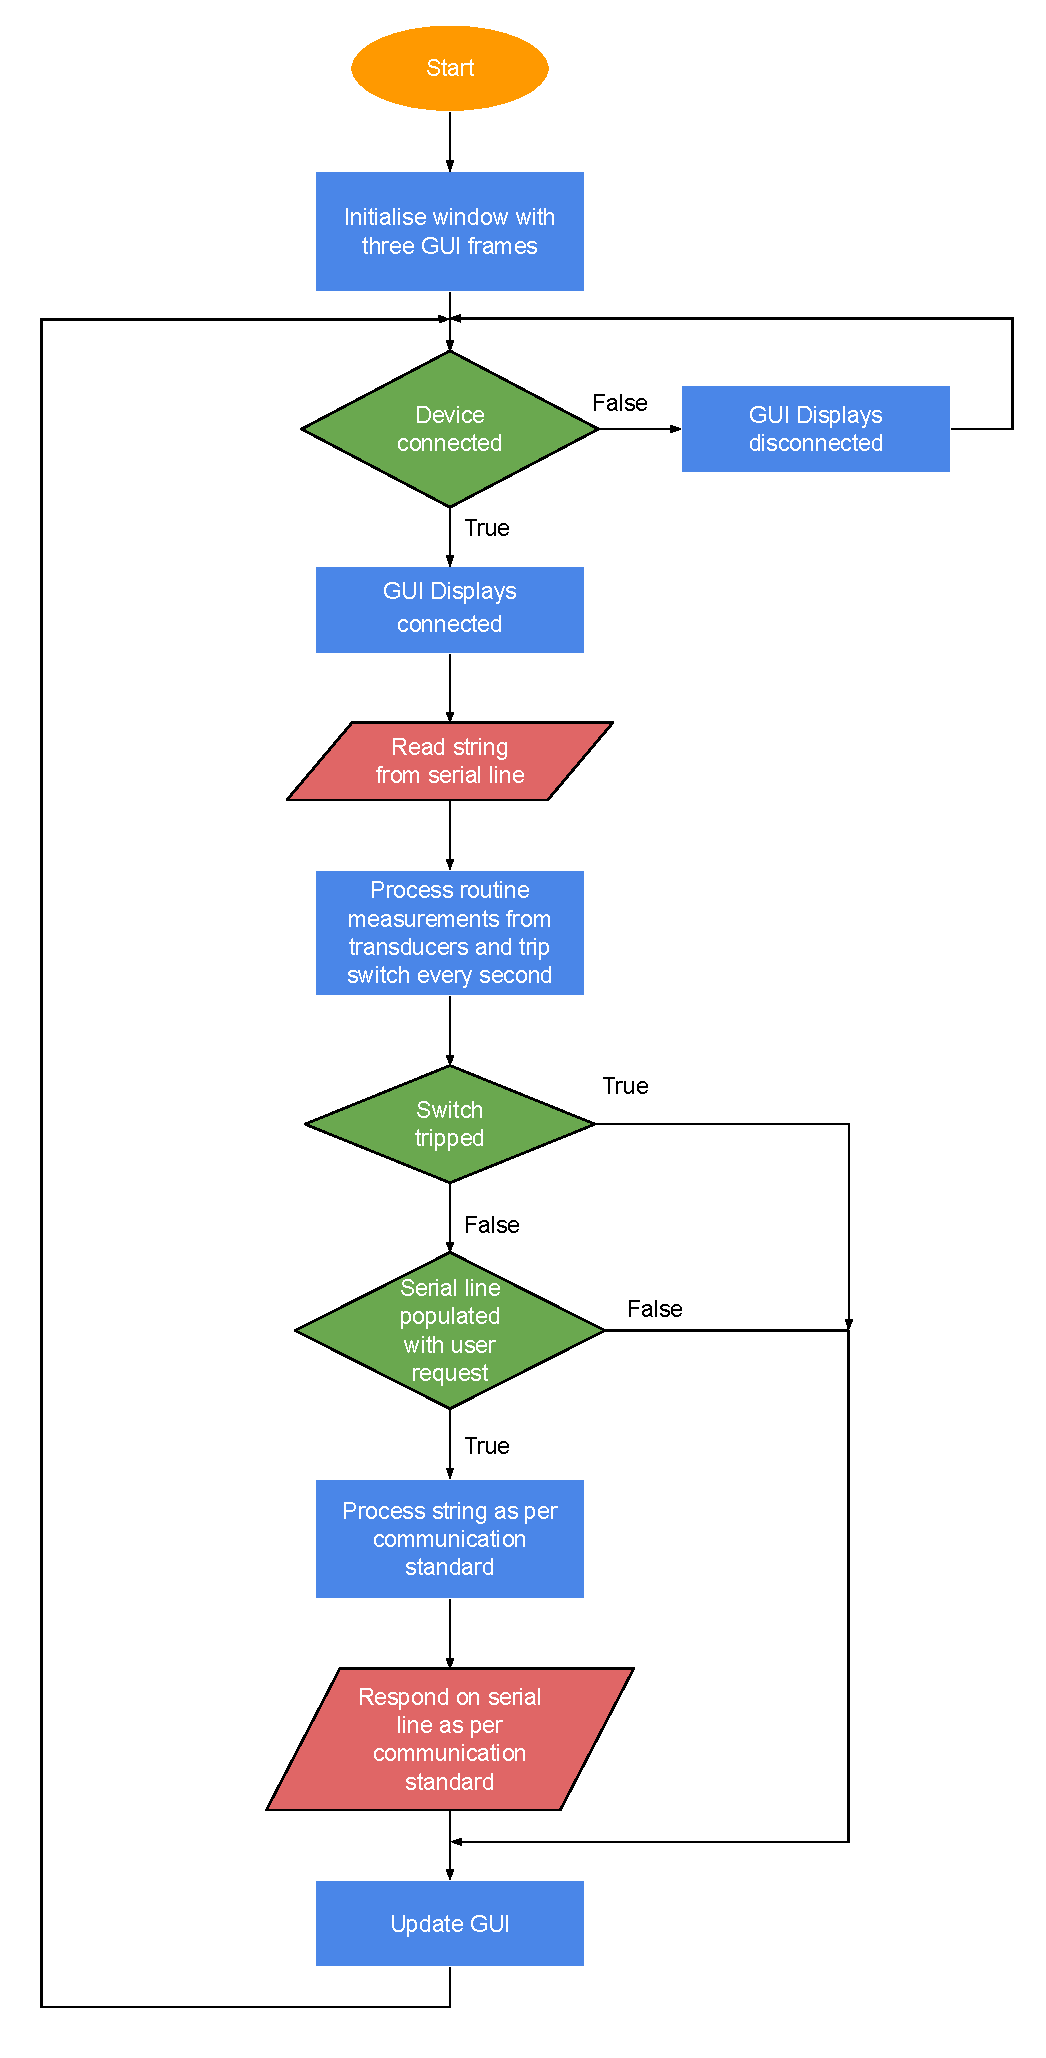
\includegraphics[width=1.0\linewidth]{./Figures/python_code_flow.pdf}
		   \caption{ } \label{subfig:python_code_flow}
     \end{subfigure}
   \caption[Flow diagram of logic for Arduino and Python code]{Flow diagram: (a) Arduino code logic. (b)  Python code logic.  }
    \label{fig:code_flow}
 \end{figure}





